\chapter{ Maximização do coeficiente \dmc utilizando matriz \pdcca~e $DPDCCA$}\label{cap:paper_03}



\begin{flushright}
    ``Noel Meyerhof consulted the list he had prepared \\
    and chose which item was to be first. \\
    As usual, he relied mainly on intuition.''\\[10px]
    (Isaac Asimov)
    % Isaac Asimov - Jokester - 1956
    \end{flushright}



\begin{figure}[!htb]
	\centering
	\caption{\dmc~de todo os canais do experimento[1:63] para cada canal como variável dependente}
	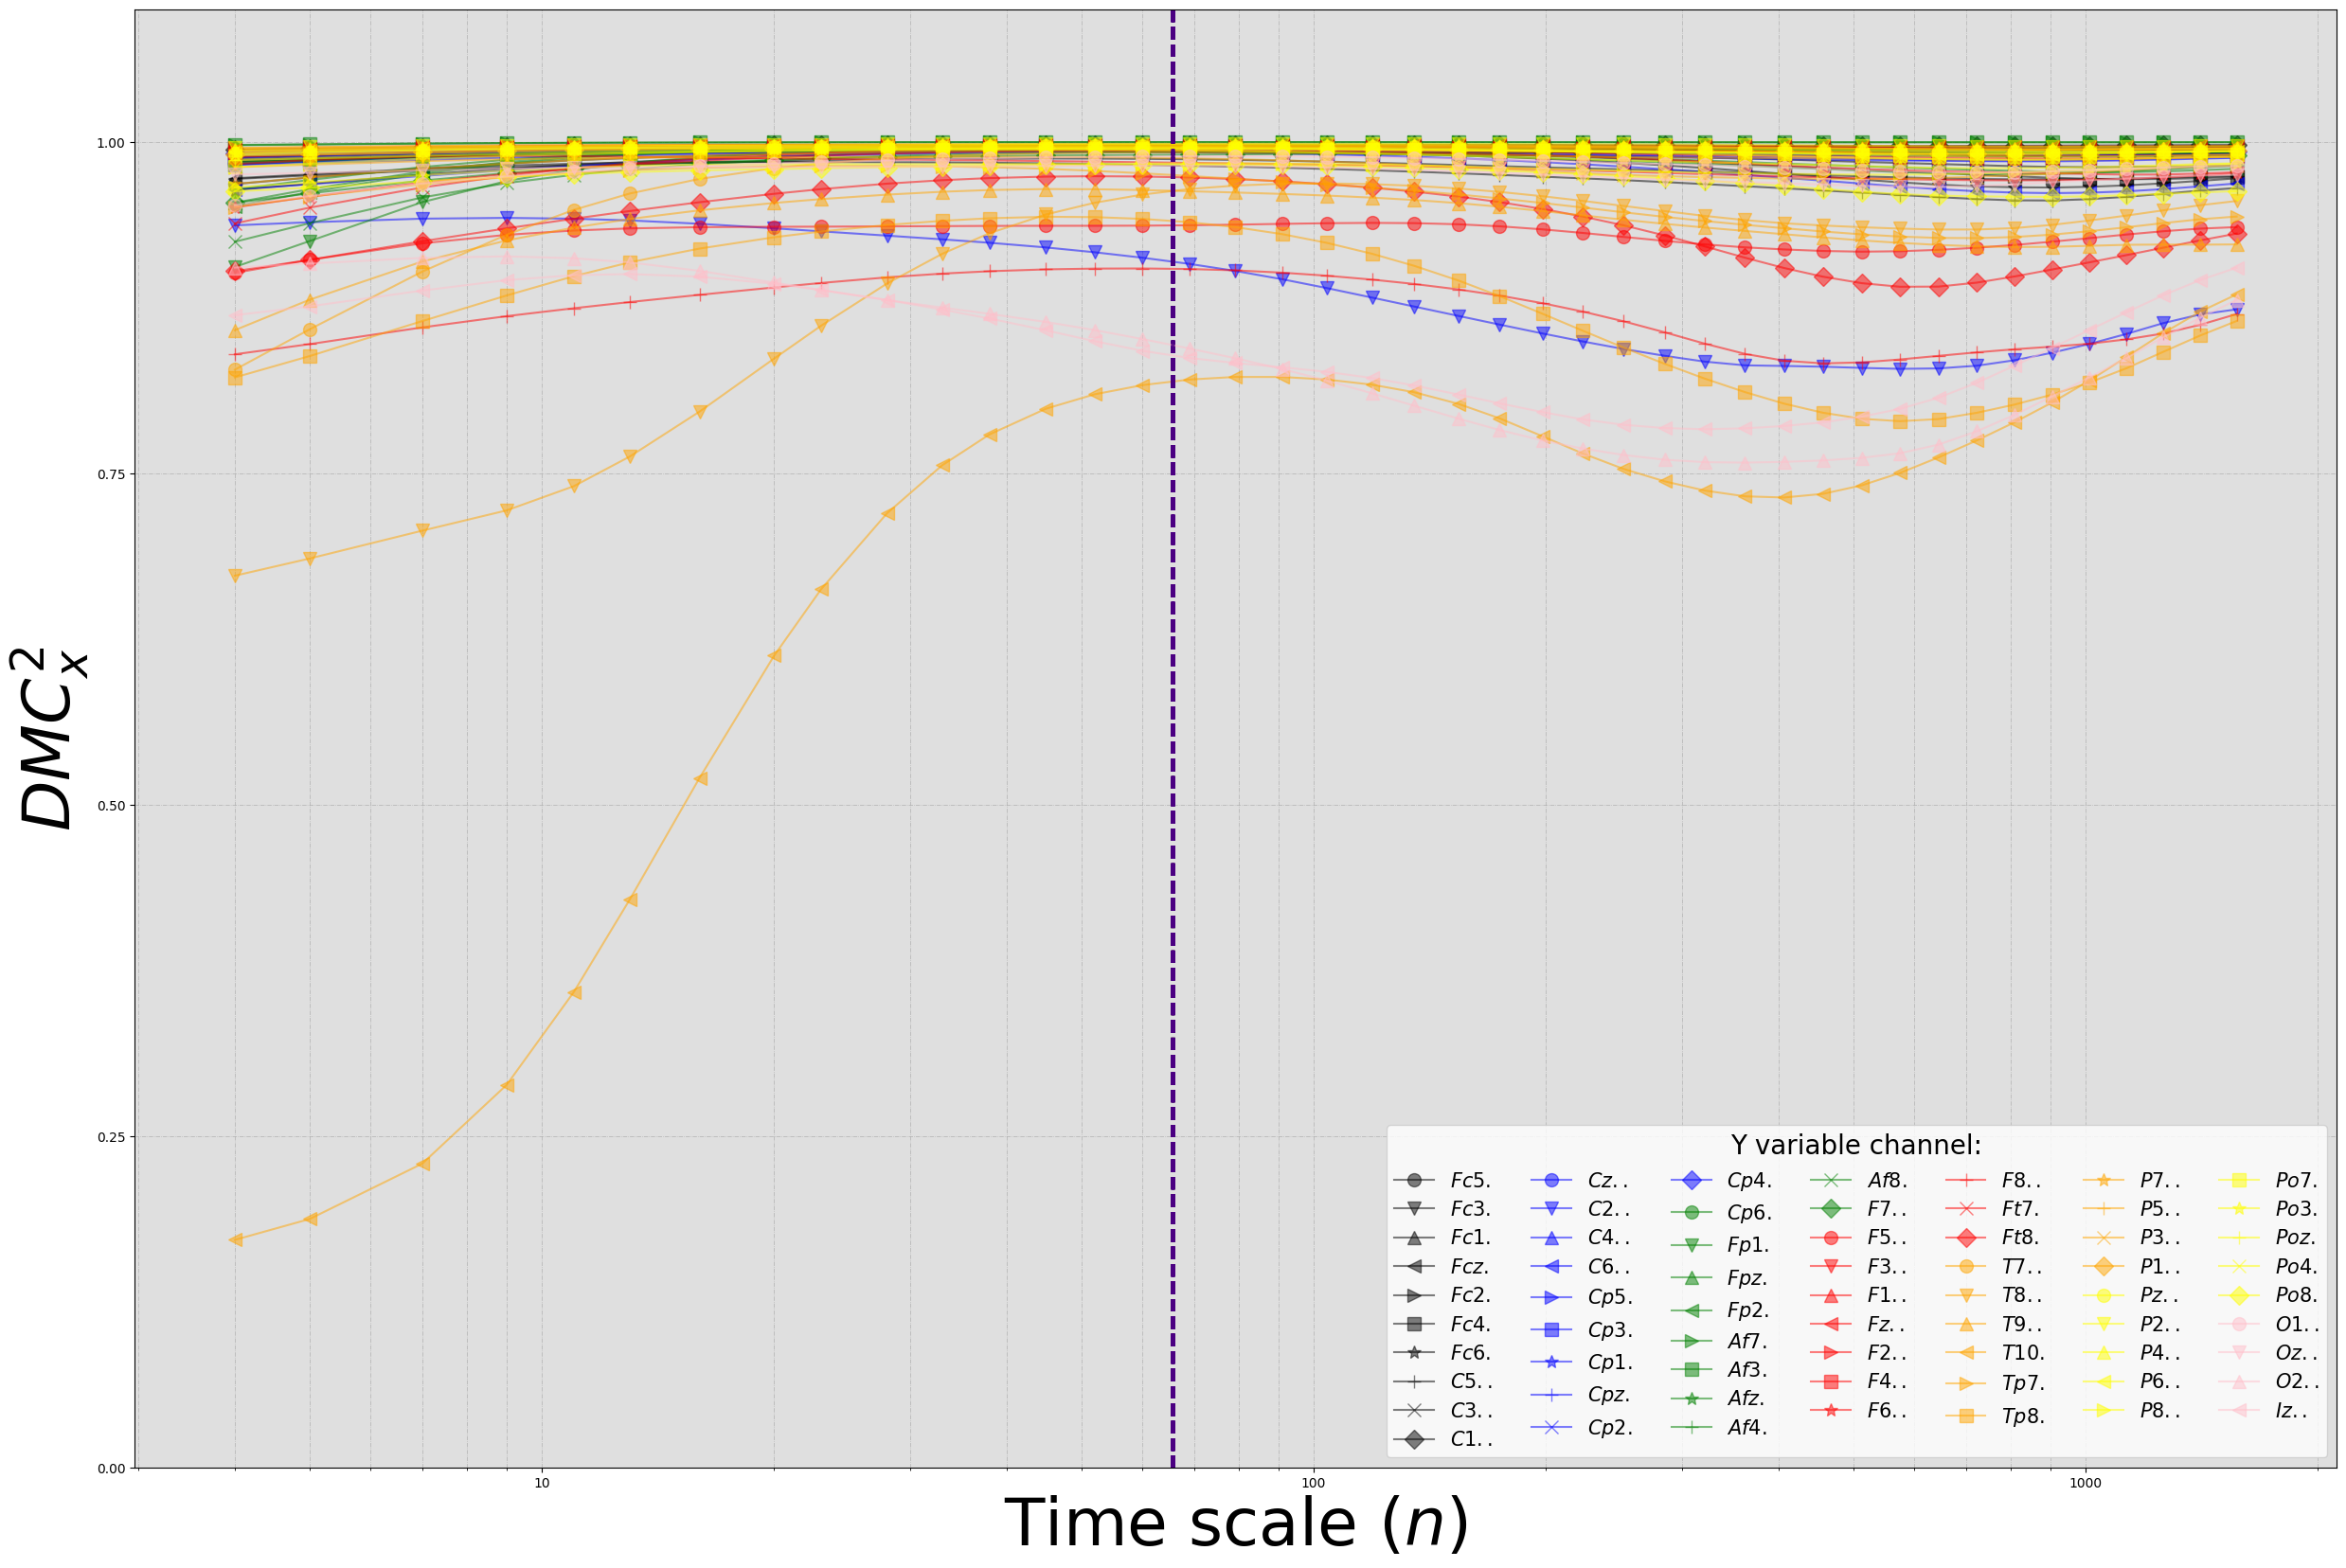
\includegraphics[width=.95\textwidth]{./Figures/art_03/dmc_all.png}
	\\{\footnotesize Fonte: Elaborada pelos autores}
	\label{fig:a03_dmc_total}
\end{figure}

Com a ferramenta desenvolvida e testada, volta-se para os dados utilizados nos artigos do Capítulo~\ref{cap:paper_01}, e no Anexo~\ref{an:a}. A matriz do \pdcca~para todos os $64$ canais é calculada em menos de $17s$. Isso se deve ao Algoritmo \emph{Detrended Saved}. Sem a aplicação deste, calculando o número de combinações necessárias para a montagem da matriz (Equação~\ref{eq:combinations_2x2}), levando em conta que, para cada \dcca~aplica-se duas vezes o cálculo do $DV$, chega-se ao valor de $2016 \times 2 = 4032$. Com o uso do algoritmo, apenas $64$ valores são calculados.

Com a matriz montada, o cálculo do \dmc, envolvendo todas as $64$ séries, com cada uma delas como variável dependente, para os $42$ valores de $n$, utilizados nos referidos artigos, é realizado em $0.7s$.

A Figura~\ref{fig:a03_dmc_total} apresenta esses resultados. Apontando para um sistema altamente correlacionado. Também encontramos um pico de correlação entre as escalas $n=60$ e $n=69$, confirmando o encontrado nos artigos.

A inversa de cada uma das $42$ matrizes do \pdcca~também foi calculada em menos de $1s$. O $DPDCCA$ foi implementado e calculado para todas as combinações de canais, levando também menos de $1s$ na execução.



\begin{table}[h!]
    \centering
    \caption{Maximização do \dmc. $n=4,~ x~len=8$, referência$= 0.6726$} \label{tab:time_4}
    \begin{tabular}{c|c|c|c}
      \hline
      Método & canais & valor & percentual \\
      \hline
      \hline
      \pdcca & T8 Fc6 C6 Cp6 F6 F8 Ft8 P4 P6 & 0.6330  & 94.1108\% \\
      $|$ \pdcca $|$ & T8 Fc6 C6 Cp6 F6 F8 Ft8 P4 P6  & 0.6330 & 94.1108\% \\
      Agg. Partial & T8 Fc6 C6 Cp6 F2 F4 F6 F8 Ft8 & 0.6329 &  94.0908\% \\
      Partial & T8 C6 Cp6 Fp2 Afz F3 F4 Ft8 P6 & 0.5686 & 84.5341\% \\
      Random & T8 F3 F1 Po7 F5 P7 Cp1 Cp4 & 0.3138 & 46.6517\% \\
      
      \hline
    \end{tabular}
  \end{table}